%
% The first command in your LaTeX source must be the \documentclass command.
\documentclass[acmlarge,screen,dvipsnames]{acmart}
%\usepackage{color}
\usepackage{amsmath}
\usepackage{pseudocode}
\usepackage[ruled]{algorithm2e}
\usepackage{algorithmicx}
\usepackage{subcaption}
\usepackage{natbib}

\input widebar

\usepackage[normalem]{ulem}  % for strike-through (\sout)
\input twmacros
%
% defining the \BibTeX command - from Oren Patashnik's original BibTeX documentation.
\def\BibTeX{{\rm B\kern-.05em{\sc i\kern-.025em b}\kern-.08emT\kern-.1667em\lower.7ex\hbox{E}\kern-.125emX}}
    
% Rights management information. 
% This information is sent to you when you complete the rights form.
% These commands have SAMPLE values in them; it is your responsibility as an author to replace
% the commands and values with those provided to you when you complete the rights form.
%
% These commands are for a PROCEEDINGS abstract or paper.
%\copyrightyear{2018}
%\acmYear{2018}
%\setcopyright{acmlicensed}
%\acmConference[Woodstock '18]{Woodstock '18: ACM Symposium on Neural Gaze Detection}{June 03--05, 2018}{Woodstock, NY}
%\acmBooktitle{Woodstock '18: ACM Symposium on Neural Gaze Detection, June 03--05, 2018, Woodstock, NY}
%\acmPrice{15.00}
%\acmDOI{10.1145/1122445.1122456}
%\acmISBN{978-1-4503-9999-9/18/06}

%
% These commands are for a JOURNAL article.
\setcopyright{acmcopyright}
\acmJournal{JOCCH}
\acmYear{2018}\acmVolume{37}\acmNumber{4}\acmArticle{111}\acmMonth{8}
\acmDOI{10.1145/1122445.1122456}

%
% Submission ID. 
% Use this when submitting an article to a sponsored event. You'll receive a unique submission ID from the organizers
% of the event, and this ID should be used as the parameter to this command.
%\acmSubmissionID{123-A56-BU3}

%
% The majority of ACM publications use numbered citations and references. If you are preparing content for an event
% sponsored by ACM SIGGRAPH, you must use the "author year" style of citations and references. Uncommenting
% the next command will enable that style.
%\citestyle{acmauthoryear}

%
% end of the preamble, start of the body of the document source.
\begin{document}

%
% The "title" command has an optional parameter, allowing the author to define a "short title" to be used in page headers.
\title[Fracturing artefacts into 3D printable puzzles]%
      {\KRedit[Digital workflow for creating 3D puzzles to engage audiences in the interpretation of archaeological artefacts]{Fracturing artefacts into 3D printable puzzles to enhance audience engagement with heritage collections}}
%
% The "author" command and its associated commands are used to define the authors and their affiliations.
% Of note is the shared affiliation of the first two authors, and the "authornote" and "authornotemark" commands
% used to denote shared contribution to the research.
\author{Karina Rodriguez Echavarria}
\email{K.Rodriguez@brighton.ac.uk}
\orcid{0000-0002-8679-1602}
\affiliation{%
  \institution{Centre for Secure, Intelligent and Usable Systems, University of Brighton}
  \city{Brighton}
  \country{United Kingdom}
}

\author{Myrsini Samaroudi}
\affiliation{%
  \institution{Centre for Secure, Intelligent and Usable Systems, University of Brighton}
  \city{Brighton}
  \country{United Kingdom}
  }

\author{Tim Weyrich}
\affiliation{%
  \institution{University College London}
  \city{London}
  \country{United Kingdom}
}


%
% By default, the full list of authors will be used in the page headers. Often, this list is too long, and will overlap
% other information printed in the page headers. This command allows the author to define a more concise list
% of authors' names for this purpose.
\renewcommand{\shortauthors}{K. Rodriguez, M. Samaroudi \& T. Weyrich}

%
% A "teaser" image appears between the author and affiliation information and the body 
% of the document, and typically spans the page. 
\begin{teaserfigure}
\centering
\subcaptionbox{3D scanned urn model\label{step1}}
 {\raisebox{0.3\height}{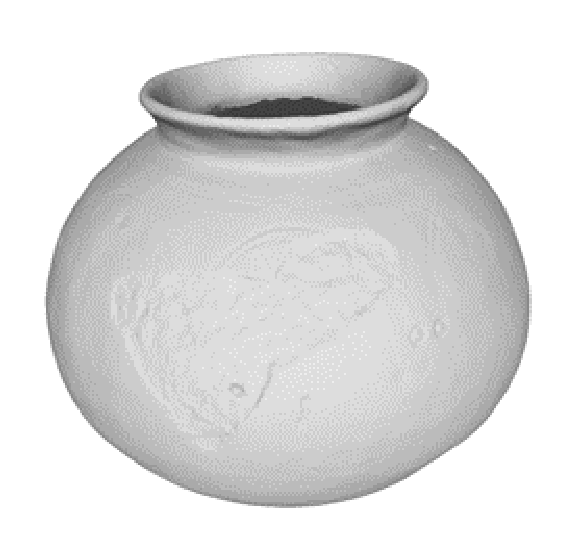
\includegraphics[width=.23\linewidth]{images/potscanned}}}
 \subcaptionbox{Generated puzzle pieces and core\label{step2}}
 {\includegraphics[width=.40\linewidth]{images/allpieces}}
 \subcaptionbox{Fabricated puzzle in museum exhibition\label{step3}}
  {\includegraphics[width=.35\linewidth]{images/exhibitmuseum}}
  \caption{Workflow for the development of physical puzzles of pottery archaeological artefacts}
  \label{fig:teaser}
\end{teaserfigure}
%
% The abstract is a short summary of the work to be presented in the article.
\begin{abstract}
\KRedit[]{Three-dimensional (3D)} puzzles of heritage artefacts are typically used to engage audiences in the
interpretation of archaeological artefacts in a museum \KRedit[exhibition]{gallery}. The reason for this is that a puzzle can be seen as \MSedit[a game]{an enjoyable educational activity in the form of a game} but also as a
complex activity that archaeologists undertake \MSedit[to re-assemble]{when re-assembling}
fragments, \MSedit[]{for instance of broken pottery}. \KRedit[]{Until now the creation of this type of experiences is mostly a manual process and the artefacts used rarely reflect those in the collection due to the obvious destructive nature of the puzzle making process. To overcome these limitations,} the contribution of this paper is a novel \KRedit[digital]{} worfklow
for the design and fabrication of 3D \KRedit[heritage]{} puzzles \KRedit[]{of artefacts}. The input to
the workflow is an authentic artefact from a heritage collection,
which is then digitised using technologies such as 3D scanning and 3D
modelling. Thereafter, a puzzle generator system produces the \KRedit[3D]{} puzzle
pieces using a cell fracture algorithm and generates a set of puzzle
pieces (female) and a single core piece (male) for
fabrication. Finally, the pieces are fabricated using 3D printing
technology and post-processed to facilitate the puzzle assembly. To
demonstrate the feasibility of the proposed novel workflow, we \MSedit[deploy the proposed method]{deployed it} to create a
puzzle exhibit of \MSedit[an artefact,]{} the Saltdean urn, \MSedit[for]{which is exhibited at} the Archaeology
Gallery of the Brighton Museum and Art Gallery. \MSedit[]{The workflow is also used with further artefacts in order to demonstrate its applicability to other shapes and types of artefacts.} The significance of
this research is that it eases the task of creating puzzle-like
activities and maintaining them \MSedit[]{in the long term} within a busy public space such as a museum gallery.
\end{abstract}

%
% The code below is generated by the tool at http://dl.acm.org/ccs.cfm.
% Please copy and paste the code instead of the example below.
%
 \begin{CCSXML}
<ccs2012>
<concept>
<concept_id>10010147.10010371.10010396</concept_id>
<concept_desc>Computing methodologies~Shape modeling</concept_desc>
<concept_significance>500</concept_significance>
</concept>
<concept>
<concept_id>10010147.10010371.10010396.10010398</concept_id>
<concept_desc>Computing methodologies~Mesh geometry models</concept_desc>
<concept_significance>100</concept_significance>
</concept>
<concept>
<concept_id>10010405.10010432.10010439.10010440</concept_id>
<concept_desc>Applied computing~Computer-aided design</concept_desc>
<concept_significance>300</concept_significance>
</concept>
<concept>
<concept_id>10010405.10010469.10010470</concept_id>
<concept_desc>Applied computing~Fine arts</concept_desc>
<concept_significance>300</concept_significance>
</concept>
</ccs2012>
\end{CCSXML}


\ccsdesc[500]{Computing methodologies~Shape modeling}
\ccsdesc[100]{Computing methodologies~Mesh geometry models}
\ccsdesc[300]{Applied computing~Computer-aided design}
\ccsdesc[300]{Applied computing~Fine arts}


%
% Keywords. The author(s) should pick words that accurately describe the work being
% presented. Separate the keywords with commas.
\keywords{cultural heritage, 3D printing, gallery design, \MSedit[]{hands-on activities, educational puzzles}}


  %\caption{a) 3D scanned model of pottery urn artefact; b) 3D model of puzzle pieces of reconstructed urn; c) printed parts of the puzzle }



%
% This command processes the author and affiliation and title information and builds
% the first part of the formatted document.
\maketitle




%-------------------------------------------------------------------------
\section{Introduction}

The technological developments over the last years in 3D printing along with the
attention that its applications have attracted from various
communities, have resulted in making digital fabrication a popular
topic of research, practice and discussion. Even though there is still
a need to deal with several related obstacles, such as design
knowledge, cost and available materials, before the widespread
adoption of digital fabrication in people's everyday lives, the
Cultural Heritage (CH) domain has proved to be a valuable field to try
digital fabrication technologies. These technologies have already been
implemented in a variety of processes in the CH sector from
conservation and exhibition planning to packaging and creative or
educational activities
\cite{Neely2013,Scopigno2014,Neumuller2014,Scopigno2015}.

This paper is concerned with the development of an application of
digital fabrication which aims to contribute to the educational and
communicational aspect of the CH experience. In particular, it
examines how digital 3D models of artefacts can be re-purposed in
creative ways in order to expand the benefits of the digitisation
process. As such, the paper proposes the playful use of a 3D puzzle to
enable users to experience the physical pieces or shards of a pot in a
similar way that archaeologists do when uncovering and synthesizing an
artefact found at an excavation site. This requires digitally breaking
a 3D shape into pieces and physically fabricating them in such a way
that the puzzle can be easily re-assembled.

The main technical contribution of this paper is a novel workflow for generating
and fabricating the 3D puzzle when the given input is an
authentic \KRedit[museum]{cultural heritage} artefact. \KRedit[]{The workflow is driven by
the requirement of being adaptable to different types of fractures and number of pieces. For instance, less number of pieces might be required if the puzzle is to be easily assembled by a young person
or child.}

\KRedit[]{An additional technical contribution of the paper is the experimentation with different fracturing algorithms for generating the puzzle pieces. The paper proposes a new algorithm which mimics the way archaeological artefacts, such as pottery, break into smaller shard pieces.} \KR{Tim, please revise this paragraph...}


\KRedit[]{In order to test the workflow, this} is deployed with a late Iron Age burial urn
from the area of Sussex (UK) - a significant object from the Brighton
Museum and Art Gallery collection. The generated puzzle \KRedit[will be]{has been}
incorporated into the Archaeology \KRedit[exhibition at the museum and is
targeted]{Gallery in order} to enhance young audiences' visiting experience while
engaging them in an educational activity.



The paper is organised as follows. Section~\ref{related} discusses
relevant work in the field including 3D printing technologies to
communicate cultural heritage information and engage
audiences. Section~\ref{requirements} introduces the particular
artefact which drove the requirements for the development of the
puzzle generating workflow and the audience of the
application. Section~\ref{workflow} then presents the proposed
workflow for the design and fabrication of the puzzle, including the
3D scanning of the artefact, its reconstruction and \KRedit[an algorithm]{the algorithms develped} for
generating the puzzle. \MSedit[]{Section~\ref{sec:fragment-generation}
  presents the results of the developed algorithms applied to other
  shapes and types of artefacts in order to demonstrate the generic
  nature of the workflow.} Section~\ref{eva} discusses the evaluation
of the application and the advantages of the adopted
approach. Finally,
section~\ref{conclusions} presents discussions and conclusions.

%-------------------------------------------------------------------------
\section{Related work}
\label{related}

\subsection{Digital fabrication to communicate CH information}

Digital fabrication technologies comprise a combination of
programmable digital tools, processes, materials and equipment which
allow the creation of physical objects of complexities not achievable
by traditional manufacturing processes.

The interest from the CH community in these technologies is high as
they offer the ability to manipulate the digital representation of an
artefact in creative ways. In addition, these technologies enable a
high-level of customisation when producing physical objects in a
variety of resolutions, materials, colours and densities. Another
important advantage of digital fabrication includes the possibility
for multiple replication and/or production in a cost-effective way,
while ``future-proofing'' the information related to the artefact
itself. Hence, these technologies are driving new trends for the
mass-customisation of CH objects and experiences.

The term ``smart'' replicas has also become popular over the recent
years. This refers to the possibility of combining the physical object
with further layers of interpretative multimedia information
\cite{Capurro2015,Marshall2016}.

Moreover, digital fabrication applications to support the
interpretation and communication of CH can be found in many heritage
organisations around the world. These examples include applications,
such as the full 3D print of the Sarcophagus of the Spouses from the
Villa Giulia Etruscan Museum, which can support visitors in having a
more holistic approach (by vision and touch) for the interpretation of
an artefact~\cite{Guidazzoli2014}.

Another example involves audiences in scanning objects and mixing 3D
models to produce hybrid artefacts by using digital fabrication. These
activities can be oriented to people with knowledge of 3D tools, such
as artists participating in 3D scanning and printing Hackathons
\cite{Mullaney2012,Neely2013}. However, some institutions
(e.g. British Museum and the Art Institute of Chicago) deploy 3D
printing in order to involve groups in workshops for non-experts. Such
groups include teachers, teenagers and families who engage with the
museums' collections through 3D technology
\cite{BritishMuseum2016,Neely2015,Miles2015}.

Other examples employ 3D printed artefacts in educational programmes
for children. The American Museum of Natural History asked students to
capture and replicate dinosaur fossils from the museum's palaeontology
collections in order to synthesise a dinosaur and learn to think like
palaeontologists~\cite{AMNH2013}. \KRedit[]{Another application is a megalithic
freestanding stone from Wales (UK) that was 3D printed in sliced vertical pieces 
that slide down a
cylindrical pillar~\cite{Miles2015}.}

Visually impaired audiences as well as the elderly constitute groups
that can also benefit greatly from digital fabrication. \cite{DAgnano2015} proposes a system which
facilitates the navigation on an architectural 3D printed facade,
allowing blind users to listen to audio descriptions. Other research deploy 
3D printed reliefs, with complementing interactive
applications, to support visually impaired users to feel paintings and
natural history exhibits~\cite{Reichinger2016a,Samaroudi2017}.

At the same time, digitally fabricated artefacts can work as
engagement vehicles for elder audiences or trauma survivors while
experiencing the ``healing'' properties of object handling and
reminiscence~\cite{PleaseTouch2016}.

Alternative uses of replicas include the production of edible
artefacts, such as the ones created at the MediaLab of The
Metropolitan Museum of Art in New York, aiming to support the
understanding of artefacts by providing a multisensorial experience to
visitors~\cite{Tang2015}. More ``traditional'' examples can be found
in museums' shops, where replicas are sold as souvenirs or
decorative/collection objects~\cite{Young2017}.

Lastly, replicas have also served purposes related to the repatriation
of original artefacts. In these cases, replicas are kept in the
possession of the organisation while the original artefact returns to
its possessor (the opposite can happen as well)~\cite{Hollinger2013}.
 
The breadth and spread of applications demonstrates i) the wide
variety of experiential frameworks to provide people with the
opportunity to ``meet'' and ``feel'' culture in alternative ways, and
ii) the potential of digital fabrication technology to support the
interpretation of a cultural heritage artefact and engage audiences. \KRedit[]{Within this context,} the development of
\KRedit[digitally fabricated]{sustainable workflows to create 3D puzzle experiences}  for audiences is a novel contribution to
the wider efforts in this area.

\subsection{Design challenges and relevant cases}
 
%This paper presents the design requirements and the workflow for the
%creation of a digitally fabricated puzzle pot.
%
The creation of a digitally fabricated puzzle can be achieved by
different methods and tools. An important overall requirement is the
generation of the puzzle pieces and the mechanism for their
assembly. The graphics' community has previously conducted relevant
research. For instance, the generation of interlocking parts from a 3D
model has been a popular topic over the last years, as it is not
currently possible to print a single object that is larger than the
working volume of a 3D printer. As such, various systems are proposed
which take as an input a 3D model and produce various smaller
interlocking pieces for 3D printing
\cite{Song:2015:POI:2797416.2797510,luo_chopper:_2012,klein_interlocking_2014,skouras_interactive_2015}. Moreover,
\cite{Xin:2011:MBP:2010324.1964992,Song:2012:RIP:2366145.2366147,sun_computational_2015}
present various algorithms for generating puzzles with interlocking
pieces, known as burr puzzles, from a 3D model.

\KRedit{Another relevant area of research is the \MSedit[]{fracturing} simulation \MSedit[of fractures for]{of} 3D models. These fracturing effects are often used to display the breaking or destruction of objects or places in
computer games, virtual reality and the film industry. In this area, predefined fracture patterns are often computed, while more novel solutions focus on creating fast approximations which are computational efficient and offer flexible control of fragment generation \cite{Schvartzman:2014:FAB:2556700.2556713,Hahn:2016:FAB:2897824.2925902,Zhu:2015:SRB:2809654.2766942,Muller:2013:RTD:2461912.2461934}. 



Moreover, most of the proposed solutions \KRedit{for creating puzzles which are 3D printable} aim to create puzzles \KRedit[]{consisting of pieces which interlock with each other, without the need to have a fixed installation.} \MSedit[However,]{In our case,} we aim to
create a permanent \MSedit[]{hands-on} exhibit \KRedit[of a pottery vase]{} for a \KRedit[]{public scape, such as a} busy museum
gallery. \KRedit{As pottery is a common archaeological finding at an excavation site, we focus on this type of artefact, and the shape of its fragments when broken into shards or pieces. This type of artefact is also interesting as its reconstruction from
shards is a problem often faced by archaeologists.}. \KRedit[This means the puzzle should be easy to assemble by providing
a clue of the overall shape, and the concave nature of the shape means
that it can wrap around a static core element.]

Of relevance to the heritage field is the geometric analysis of a dataset of fracture patterns observed in wall paintings excavated at Akrotiri, Greece~\cite{Shin:2012:ASF:2362402.2362404}. This analysis suggests that when pottery is broken, this fragments in a hierarchical fracture pattern, where fragments break into two pieces recursively along cracks nearly orthogonal to previous ones.}


Similar examples of pottery puzzles in other museums (though without
deploying a fully digital workflow) are shown in
Figure~\ref{fig:puz}. As shown in the images, these puzzles require a
static element (the core) that \MSedit[provides a clue of]{might provide clues about} the overall shape of
the pot. Moreover, the core helps \KRedit[the user to assemble the puzzle]{to secure the pieces in place} with
the use of magnets \KRedit{or other attachment mechanisms which are placed both} on \KRedit[its]{the core's} surface and on each puzzle piece. An initial proposal for a digital workflow to generate this type of puzzles is present in \cite{01763a4734614c50ab9f408cdd0f5470}. This paper extends the digital workflow to incorporate different fracture patterns as well as presents a full deployment of the workflow on an exhibit of the Brighton Museum and Art Gallery.


\begin{figure}[H]
  \centering
  \subcaptionbox{Puzzle-pot from the Bristol Museum \& Art Gallery (UK), photo courtesy of Andrew Maxted}
  {\includegraphics[width=0.35\linewidth]{images/uk}}
  \hspace{0.5in}
  \subcaptionbox{Puzzle-pot from Rez\'e Museum (France), photo courtesy of Theophane Nicola}
  {\includegraphics[width=0.35\linewidth]{images/france}}
  \caption{\label{fig:puz}Examples of pottery puzzles in museums}
\end{figure}




%Also, both the core and puzzle pieces are 3D printed making the exhibit and activity ``future-proof''. 
%Lastly, away from the puzzle context,~\cite{Barreau2014} propose a workflow to reconstruct a broken pot in order to display the existing shards for exhibition purposes.

\KRedit[The contribution of this paper is the proposed workflow to generate a
3D puzzle of a pot, which is a popular type of archaeological
artefact. This particular type of object is interesting as it is
widely found in all historic societies and its reconstruction from
shards is a problem often faced by archaeologists. The following
section will present more details on the particular object and the
design of the experience.]


%-------------------------------------------------------------------------
\section{The 3D puzzle experiential framework}
\label{requirements}
\KRedit[A funerary urn, shown in Figure~\ref{fig:pot}, from the collection of
the Brighton Museum and Art Gallery has been selected in order to
design an experience that will engage young audiences in assembling a
digitally fabricated 3D puzzle of the urn's replica.]{The motivation to develop the proposed workflow stemmed from the need to design an \MSedit[experience]{experiential framework} that \MSedit[will]{would} engage young audiences with the archaeological collection of the Brighton Museum and Art Gallery. Thus, the requirement was to design a 3D puzzle of a funerary urn, shown in Figure~\ref{fig:pot}.}
 The urn comes
from the cliff top at Saltdean, a coastal area near Brighton in
Sussex, UK. The pot has curvilinear designs which are usual in Sussex
in the two centuries BC, before the arrival of the Romans. The urn is
mostly brown and it seems that burnishing had been applied to its
surface to give it a ``leathery'' appearance. The Saltdean funerary
urn is a late Iron Age pot (probably 1st century BC) which was thrown
on a wheel~\cite{Toms1912}. It possibly reflects influences from
Belgian tribes and people from Brittany who had moved into the area
and introduced the use of the potter's wheel in south
Britain~\cite{Harding1974,Cunliffe1978,Adkins1982,Cunliffe1995}.
%
\begin{figure}[H]
  \centering
  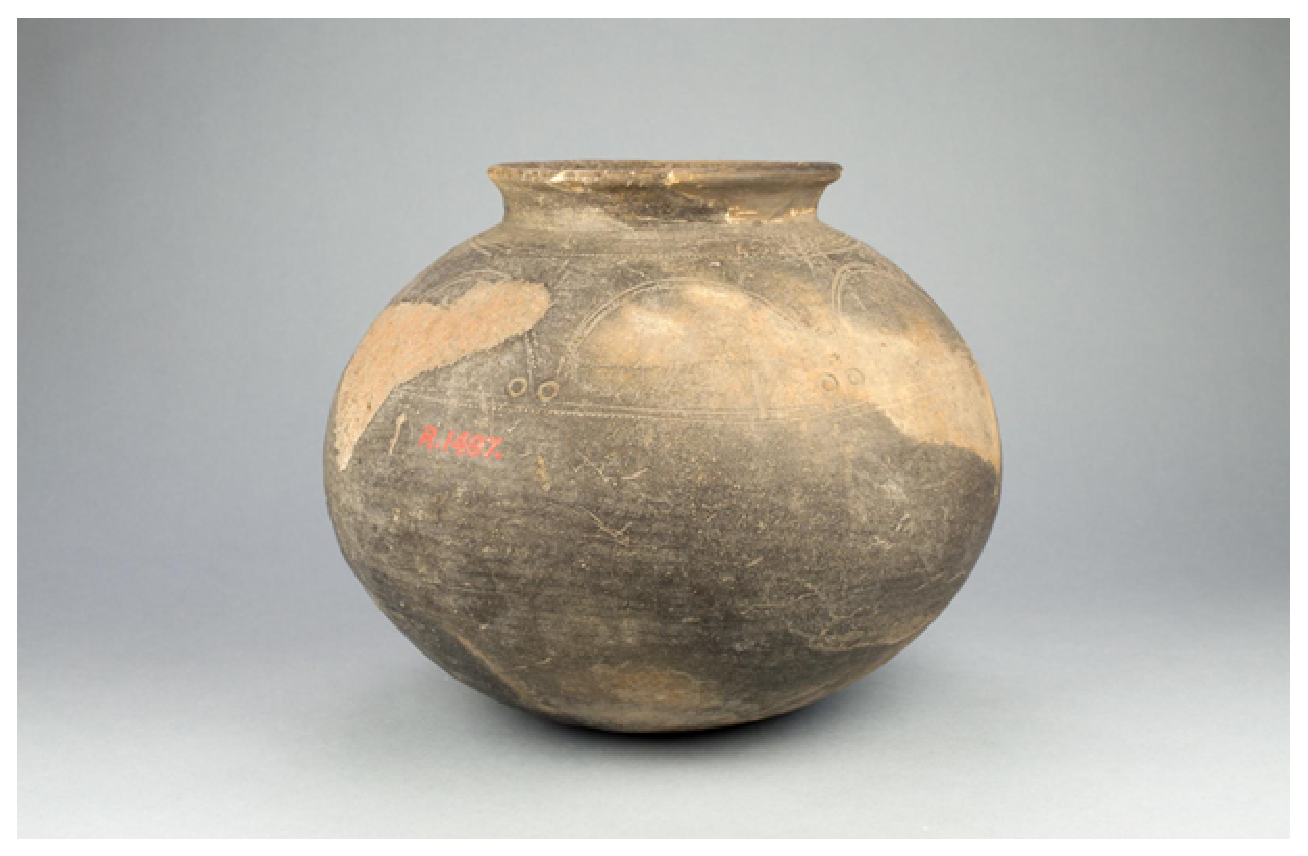
\includegraphics[width=0.6\linewidth]{images/pot}
  \caption{\label{fig:pot}
    Late Iron Age funerary urn from Saltdean, Sussex (UK)}
\end{figure}

\KRedit[The 3D puzzle will be a hands-on activity incorporated in the
Archaeological Gallery of the Brighton Museum and Art Gallery. The
puzzle will be placed along local findings of the Iron Age period and
will be close to the original artefact.]{ The
puzzle was designed to be placed as a hands-on activity along \MSedit[]{with} local findings of the Iron Age period and close to the original artefact in the new Archaeology Gallery.} The objective \MSedit[for]{of} the \KRedit[development of the puzzle]{hands-on activity} is to support young
audiences, and especially children, in having an interactive experience with a heritage artefact in the form of an educational
activity or game. \MSedit[It]{The puzzle} \KRedit[will] also allows wider audiences to experience the
challenges linked to archaeological processes, such as reconstructing
a shape from a given group of shards or pieces. By assembling the
puzzle, audiences will engage with the exhibit, its physicality,
function and history, while acquiring new skills and gaining a better
understanding about the artefact itself.

\subsection{Requirements for the production of the digitally fabricated 3D puzzle}

The main design requirements with respect to the 3D puzzle were agreed
between the researchers and the exhibition designers taking into
account design guidelines about children's
puzzles~\cite{Smith2002}. These requirements included:
%
\begin{enumerate}
\item to have the urn height scaled-up to around 300 mm (the rest of
  the dimensions of the artefact were scaled-up proportionally);
\item to have a thickness of around 10 mm for each individual piece,
  as this was found suitable for easy handling by small hands;
\item to have approximately 10-12 pieces to assemble the puzzle. Thus,
  pieces should measure at least 50.8 mm across, as 6-8 year olds can
  handle pieces of this size;
\item to design a core piece which \MSedit[will]{would} be attached to a rotating
  wooden plate so that the user can easily spin the puzzle core to
  facilitate interaction (see Figure~\ref{fig:alexdesign});
\item to enable attachment of the individual puzzle pieces to the core
  via magnets. The magnets are inserted in blind holes in the puzzle
  pieces and in the solid core. The blind holes require to be in
  predetermined matching positions both in the pieces and core;
\item to cover each individual piece in a plaster-like finish and
  paint it to disguise the magnets, provide better texture feeling and
  \MSedit[a more realistic appearance]{an appearance that would be as close as possible to the original one}.
\end{enumerate} 

\begin{figure}[H]
  \centering
  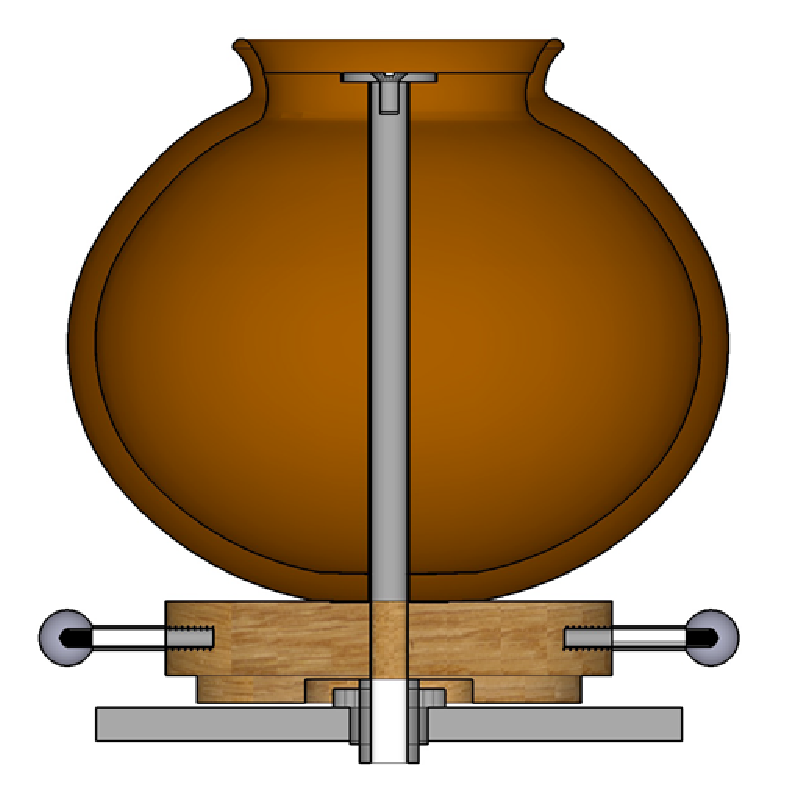
\includegraphics[width=0.5\linewidth]{images/alexdesign}
  \caption{\label{fig:alexdesign}%
    Design of puzzle core piece on its rotating base, design courtesy of Alex Hawkey}
\end{figure}

When discussing with the designer of the museum, it was acknowledged
that such requirements could be addressed by using alternative
mechanisms to digital fabrication technologies providing similar
durability and quality. However, it was deemed that the digital
workflow \MSedit[will]{would} enable to future-proof such exhibit for replacing parts
in a cost-effective manner.

\subsection{Audience}

The target group for this puzzle activity is young people, in
particular children between the age of 6 and 12 years old. This age
frame is considered as appropriate in terms of integrating a specific
type of interpretation as interpretative means can be different for
younger or older children~\cite{Tilden1977}.

The selection of this particular group, whether it is families or
school children visiting the museum, has been recognised as an
important part of most CH organisations' audiences. Children appear to
be amongst the people who can benefit the most from CH experiences
with the deployment of replicas~\cite{Cabral2013,Neely2015,Miles2015}.

Furthermore, official numbers (in the ``Overview of data in the
Museums, Libraries and Archives Sector''~\cite{Matty2004}) confirm
that most people who visit a museum/CH institution in the UK belong to
a family group or a school group. Hence, the Brighton Museum and Art
Gallery has a high number of families and school children visiting
its premises. Moreover, a survey which recorded
visitors' opinions on the potential to exhibit the archaeological
collections of the museum revealed that people would be interested in
hands-on children's activities~\cite{RoyalPavilionandMuseums2015}.

The following section will describe a digital fabrication workflow to
produce the 3D puzzle according to the specified requirements, along
with a proposed algorithm to semi-automate the design of such 3D
puzzles.

\section{Workflow for generating and fabricating a
  3D~puzzle of an artefact}
\label{workflow}

The proposed workflow involves the following steps:
%
\begin{enumerate}
\item \KRedit[Acquiring]{Digitisation} and \MSedit[reconstructing]{reconstruction of} the digital 3D model of the artefact and \MSedit[]{its} central core piece.
\KRedit{\item Generation of fracture pattern.}
\item Generation of the individual puzzle pieces.
\item Generation of \KRedit[matching blind-holes]{attachment mechanisms, such as matching blind holes,} both in the core and puzzle pieces.
\item 3D printing all puzzle pieces and core.
\item Post-processing of all puzzle pieces and core\KRedit[, which includes
  inserting the magnets]{, including adding attachments and painting.}
\item Assembling the puzzle into the final exhibit.
\end{enumerate}
%

\KRedit{The approach for \MSedit[generating]{producing} solid surfaces for fabrication, which underlies the proposed \MSedit[workshop]{workflow}, deploys algorithms that combine triangular mesh representations with constructive solid geometry (CSG) operations. CSG is a technique commonly used in solid modelling CAD systems. It allows to create a complex surface by using Boolean operators to combine simpler objects. 

The implementation of the workflow uses a mixture of tools and systems including modelling tools, C++ and OpenSCAD.  OpenSCAD is a free Computer Aided
Design (CAD) software which uses the Computational Geometry Algorithms
Library (CGAL) as its constructive solid geometry (CSG) engine. Its
script syntax is based upon functional programming philosophy which
allows to generate geometry using a functional approach.

The following subs-sections will describe each of the workflow stages in detail using the Saltdean pot as an example artefact.}


\KRedit[The following subs-sections will describe each of these stages in detail.]{}

\subsection{\KRedit[Acquiring the digital 3D model]{Digitisation and reconstruction of the} artefact}

The acquisition of an artefact can be achieved through different
means, including 3D scanning and photogrammetry techniques. In this
case, the urn was scanned using the AICON Breuckmann 3D SmartScan
scanner. Given the shape of the urn with the narrowed neck above its
rounded body, the 3D scanning process captured the external surface of
the pot, but it was not possible to acquire the internal surface. The
resulting 3D model is shown in Figure~\ref{fig:teaser}-a after some
small holes were filled in.

In order to reconstruct the internal part of the urn which was not
acquired by the scanner, it was considered that the best approach was
to solidify the external wall \KRedit[at a suitable]{with a 10 mm} thickness using the 3D 
modelling tool Blender. Before doing this, the 3D model was scaled-up
to have a 300 mm height according to the design requirements. \KRedit[Then,
using the physics capabilities of Blender to simulate real-world
phenomena, the 3D model of the urn (whose base is not completely
straight) was placed on a plane in order to acquire a standing
position (see Figure~\ref{fig:blender}). Then, the top of the urns rim was removed in order to isolate the external shell of the urn.]{The resulting  3D model which \MSedit[will be]{has been} used as input for the puzzle is shown in
  Figure~\ref{fig:reconstructiona}}.
%
% \begin{figure}[h]
%   \centering
% % 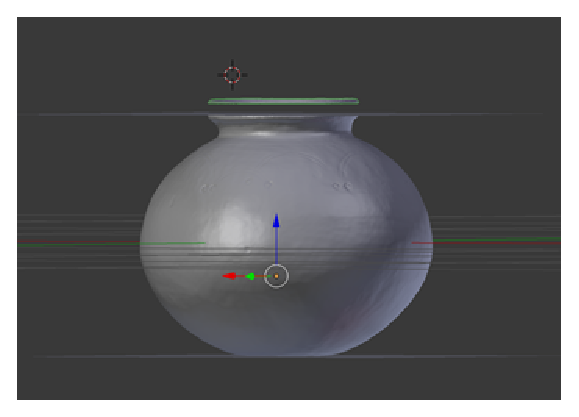
\includegraphics[width=0.45\linewidth]{images/blender1}
%   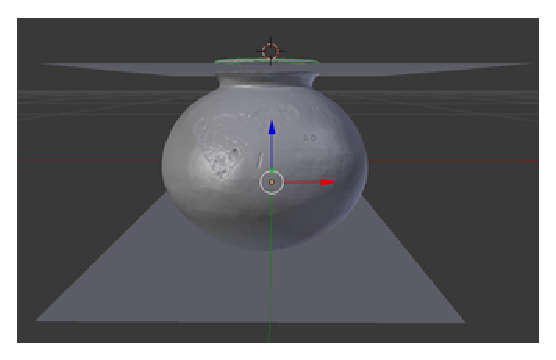
\includegraphics[width=0.6\linewidth]{images/blender2}
%   \caption{\label{fig:blender}
%     Perspective view of the urn with separated rim in Blender}
% \end{figure}

\KRedit[Subsequently, the external shell was solidified with a 10 mm thickness in Blender. This thickness is proportionally close to the scaled-up measurements of the artefact. Afterwards, two 3D models were produced:]{}

\KRedit[The urn without rim. The rim was later joined again with the urn and modeled to have a smooth feeling in order to produce the reconstructed 3D model of the pot (see  Figure~\ref{fig:reconstructiona}).]{}

\KRedit[The internal shell of the pot which constitutes the core of the puzzle. Thus, the faces of the internal shell were inverted it Meshlab and a plane was added to the top of the shape to create a watertight core (see Figure~\ref{fig:reconstructionb}).]{Afterwards, the central core piece \MSedit[is]{was} produced. This can be generated for any type of pottery puzzle by using a boolean operation. The resulting watertight model is shown in Figure~\ref{fig:reconstructionb}. The core \MSedit[requires]{required} also of a through-hole along its height in order to fit \MSedit[it to]{onto} the revolving base, as shown in the design in Figure~\ref{fig:alexdesign}.}

\begin{figure}[h]
  \centering
  \subcaptionbox{3D model of the reconstructed urn\label{fig:reconstructiona}}
  {\includegraphics[width=0.45\linewidth]{images/potcomplete}}
  \subcaptionbox{3D model of internal core of the puzzle\label{fig:reconstructionb}}
  {\includegraphics[width=0.45\linewidth]{images/corewhole}}
  \caption{3D models used for puzzle generation}
\end{figure}

\greenBegin

\subsection{Generation of fracture patterns}
\label{sec:fracture-patterns}

Before creating individual ``puzzle pieces'' (pottery
shards/fragments), we need to determine suitable fragment shapes, that
is, hypothetical fracture lines along which the ceramic object broke.

We model fracture lines within the spherical domain, conceptually
projecting the pot's geometry onto a sphere. While this restricts us
to roughly-spherical objects, it appears a reasonable approximation in
our context.

In this work, we investigated two different ways to generate such
fractures: \emph{Voronoi tessellation} of the sphere, and
\emph{hierarchical fracture} along ragged curves on the sphere.

\paragraph{Voronoi tessellation.}
%
In this approach, we generate a random set of $n$ uniformly
distributed centroids on the sphere. Fracture lines are then defined
as the edges of the corresponding spherical Voronoi diagram.
%
The resulting fragment shapes are generally more uniform than
naturally occurring pottery fragments but represent an interesting
puzzle challenge due to the higher similarity amongst fragments.
%
Figure~\ref{fig:fracture-type-examples:voronoi} shows an example set
of spherical Voronoi fragments, visualised as solid spherical sectors.

\paragraph{Hierarchical fracture.}
%
While real-world fracture lines are shaped by complex processes,
including impact geometry and volumetric distribution of
inhomogeneities in the material, Shin et al.\ in their study of
wall painting fragments~\cite{Shin:2012:ASF:2362402.2362404} found
evidence that fracture patterns have similar statistics as cracks
created by hierarchical fracture
processes~\cite{Bohn:2005:Four}.
%
This inspired our second fracture generation method that
hierarchically subdivides the spherical domain until a target number
of fragments is reached. In each iteration, one fragment is subdivided into 
two fragments by generating fracture lines at random orientations. 
Fracture lines are fractal curves to add more realistically looking raggedness 
to each edge. The method takes into account various criteria for fragmentation, including to prioritise larger fragments as well as to avoid creating very thin 
or small fragments. 

%
See Appendix~\ref{apx:hierarchical-algo} for
more details on the algorithm.  Parameters of the algorithm are shown in
Table~\ref{tab:hierarchical-parameters}.
%
\begin{table}
  \begin{tabular}{|l|p{0.933\linewidth}|}
    \hline
    \multicolumn{2}{|l|}{Hierarchical Splitting}\\
    \hline
    $N$ & Number of fragments to be produced.\\
    $r$ & Maximum area ratio between larger and smaller half of a split fragment ($r=4$ in all of our experiments).\\
    \hline
    \multicolumn{2}{l}{~}\\[-1.33ex]
    \hline
    \multicolumn{2}{|l|}{Fractal Generator}\\
    \hline
    $m$ & Initialises fracture fractal with $m$-sided spherical polygon along a great circle.\\
    $n$ & Number of recursive bisections of polygon edges.\\
    $R$ & Random jitter of polygon vertices along the great circle, as multiples of edge length.\\
    $A$ & Amplitude (as multiples of edge length) by which that polygon is tangentially displaced away from the great circle.\\
    % formally niter:
    % formally decay:
    $\rho$ & Fractal decay: $\rho=1$ creates fractal curves that are
    self-similar across all scales; values of $0 < \rho < 1$ attenuate both
    $R$ and $A$ toward finer scales.\\
    $\sigma$ & $\sigma\in[0,1]$ denotes strength of additional smoothing of the result at its finest scale.\\
    \hline
  \end{tabular}
  \caption{\label{tab:hierarchical-parameters}%
    Parameters of our hierarchical fracture algorithm.
    %
    See Appendix~\ref{apx:hierarchical-algo} for algorithmic details.}
\end{table}
%
Figure~\ref{fig:fracture-type-examples:hierarchical:first}--\ref{fig:fracture-type-examples:hierarchical:last}
shows resulting fracture line characteristics for different parameter values. Figure~\ref{fig:fracture-type-examples:hierarchical:first} demonstrates a fragmentation with a low amplitude $A$ and medium fractal decay $\rho$ to produce fragments with straight edges. Moreover, figure~\ref{fig:fracture-type-examples:hierarchical:last} demonstrates a fragmentation with a higher amplitude $A$ and a lower random jitter of polygon vertices $R$ to produce fragments with higher raggedness.

%Downside: distribution and size of fragments is harder to control. In our experiments,

\begin{figure}[H]
  \centering%
  \subcaptionbox{\label{fig:fracture-type-examples:voronoi}%
    Voronoi fracture pattern}%
  {\includegraphics[width=0.30\linewidth]{images/fractureBlender}}%
  \hspace{0.2in}%
  \subcaptionbox{\label{fig:fracture-type-examples:hierarchical:first}%
    Hierarchical fracture pattern, $m$: 6, $n$: 6, $R$: 0.3, $A$: 0.01, $\rho$: 0.5, $\sigma$: 0.0}%
  {\includegraphics[width=0.30\linewidth]{images/fracturelowamplitude}}%
  \hspace{0.2in}%
  \subcaptionbox{Hierarchical fracture pattern, $m$: 6, $n$: 6, $R$: 0.3, $A$: 0.1, $\rho$: 0.5, $\sigma$: 1.0}%
  {\includegraphics[width=0.30\linewidth]{images/fracturestandardsmooth}}%
  \hspace{0.2in}\\
 \subcaptionbox{Hierarchical fracture pattern, $m$: 6, $n$: 6, $R$: 0.3, $A$: 0.2, $\rho$: 0.2, $\sigma$: 1.0}%
  {\includegraphics[width=0.30\linewidth]{images/fracturehighamplitude}}%
  \hspace{0.2in}%
  \subcaptionbox{\label{fig:fracture-type-examples:hierarchical:last}%
    Hierarchical fracture pattern, $m$: 6, $n$: 6, $R$: 0.1, $A$: 0.3, $\rho$: 0.5, $\sigma$: 0.3}%
  {\includegraphics[width=0.30\linewidth]{images/fracturehighestamplitude}}%
  \caption{\label{fig:fracture-type-examples}%
    Fracture patterns}
\end{figure}

\greenEnd
\begin{figure}[H]
  \centering
  \subcaptionbox{3D model contained within all fragments of sphere\label{fig:spherea}}
  {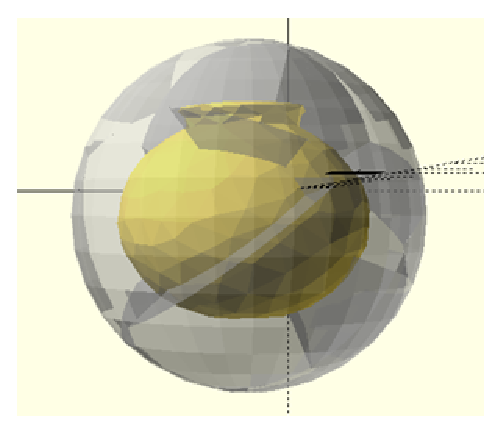
\includegraphics[width=0.30\linewidth]{images/sphere}}
  \hspace{0.2in}
   \subcaptionbox{3D model of reconstructed urn with fragment of the fractured sphere\label{fig:sphereb}}
   {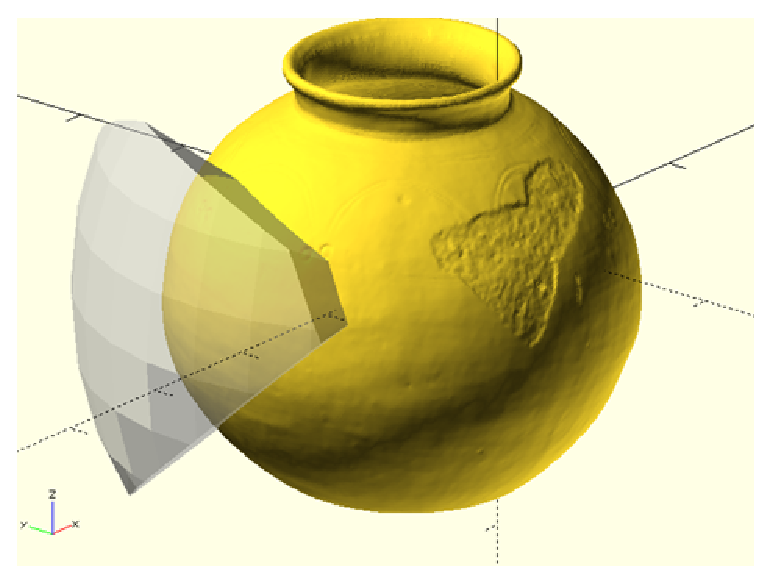
\includegraphics[width=0.30\linewidth]{images/intersection}}
   \hspace{0.2in}
  \subcaptionbox{Resulting 3D model of puzzle piece\label{fig:spherec}}
  {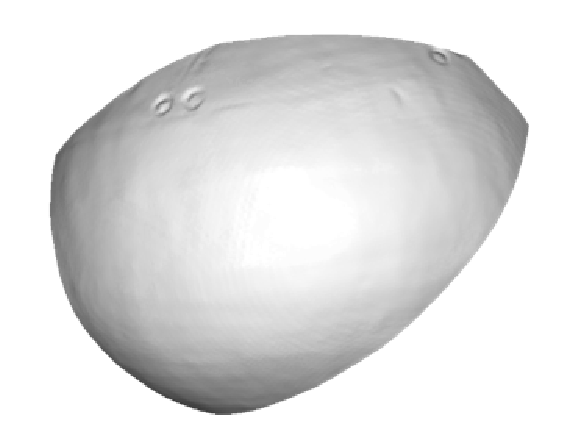
\includegraphics[width=0.30\linewidth]{images/puzzlepiece}}
    
    
    \caption{Puzzle fragment generation through CSG operations between a 3D model and the fracture pattern}
\end{figure}
\subsection{Generating the individual puzzle pieces}
\label{sec:fragment-generation}


\begin{figure}[H]    
     \centering
       \subcaptionbox{$m$: 6, $n$: 6, $R$: 0.3, $A$: 0.1, $\rho$: 0.5, $\sigma$: 0.0\label{normal}}
         {\includegraphics[width=0.33\textwidth]{images/pott1}}
      \subcaptionbox{$m$: 6, $n$: 6, $R$: 0.3, $A$: 0.1, $\rho$: 0.5, $\sigma$: 1.0\label{normalsmooth}}
        {\includegraphics[width=0.33\textwidth]{images/pott2}}
      \subcaptionbox{$m$: 6, $n$: 6, $R$: 0.3, $A$: 0.01, $\rho$: 0.5, $\sigma$: 0.0\label{lowjitter}}
        {\includegraphics[width=0.33\textwidth]{images/pott3}}
      \subcaptionbox{$m$: 6, $n$: 6, $R$: 0.3, $A$: 0.2, $\rho$: 0.2, $\sigma$: 1.0\label{highjitter}}
        {\includegraphics[width=0.33\textwidth]{images/pott5}}
      \caption{\label{fig:pot-with-different-fracture-settings}%
        Examples of puzzles with different parameters.}
\end{figure}

\begin{figure}[H]
  \includegraphics[width=0.33\textwidth]{images/ambercuppuzzle0}%
  \includegraphics[width=0.33\textwidth]{images/saltdeanpuzzle0}%
  \includegraphics[width=0.33\textwidth]{images/elephantpuzzle0}\\
  \includegraphics[width=0.33\textwidth]{images/ambercuppuzzle2}%
  \includegraphics[width=0.33\textwidth]{images/saltdeanpuzzle1}%
  \includegraphics[width=0.33\textwidth]{images/elephantpuzzle1}\\
  %\includegraphics[width=0.55\textwidth]{ambercuppuzzle3}\\
  \includegraphics[width=0.33\textwidth]{images/ambercuppuzzle4}%
  \includegraphics[width=0.33\textwidth]{images/saltdeanpuzzle2}%
  \includegraphics[width=0.33\textwidth]{images/elephantpuzzle2}\\
  \includegraphics[width=0.33\textwidth]{images/ambercuppuzzle5}%
  \includegraphics[width=0.33\textwidth]{images/saltdeanpuzzle3}%
  \includegraphics[width=0.33\textwidth]{images/elephantpuzzle3}\\
  \includegraphics[width=0.33\textwidth]{images/ambercuppuzzle6}%
  \includegraphics[width=0.33\textwidth]{images/saltdeanpuzzle4}%
  \includegraphics[width=0.33\textwidth]{images/elephantpuzzle4}
  \caption{\label{fig:three-shapes-with-different-fractures}%
    Examples of algorithm applied to scans of an amber cup, Saltdean pot and
    ceramic elephant figurine.}
\end{figure}



\KRedit[In order to generate the puzzle pieces, a semi-automated approach was
deployed using OpenSCAD software. OpenSCAD is a free Computer Aided
Design (CAD) software which uses the Computational Geometry Algorithms
Library (CGAL) as its constructive solid geometry (CSG) engine. Its
script syntax is based upon functional programming philosophy which
allows to generate geometry using a functional approach.]{}

\KRedit[The proposed approach takes as input the watertight 3D models of the
reconstructed urn (Figure~\ref{fig:reconstruction}-a) and core
(Figure~\ref{fig:reconstruction}-b), both generated in the previous
steps. The generator then produces:]{Once the fracture pattern has been generated, \MSedit[this]{it} is used to \MSedit[generate]{produce} the puzzle pieces.} \KRedit[Boolean operations are used for generating the puzzle pieces and the
internal core with matching blind holes. These sets of operations,
including union, intersection and difference, are the basis of how
geometries are constructed in CAD systems.]{} For this, CSG operations are used to generate all the printable puzzle pieces. Firstly, the 3D model is translated to the centre of the fractured
sphere (see Figure~\ref{fig:spherea}). Thereafter, as shown in
Figure~\ref{fig:sphereb}, each \MSedit[section of the fractured sphere]{fracture of the sphere}
is intersected with the 3D model of the artefact. The
intersection region of these two objects is defined as the set of all
points that are part of both objects. As a result, a puzzle piece is
produced as shown in Figure~\ref{fig:spherec}.
%

%

The algorithm iterates over all sections of the fractured sphere to
automatically produce all puzzle pieces. This process is repeated to
generate puzzle pieces at two different levels of detail so that they
can be used in subsequent operations.
  
\KRedit[]{Figures~\ref{fig:pot-with-different-fracture-settings} illustrate the 
generation of alternative versions of puzzles pieces for the Saltdean urn using various level of raggedness for similarly-sized fragments. For the museum gallery, we generated 16 individual puzzle pieces using straight edges based on the Voronoi approach as this was deemed to be the simpler version for children to complete.} \MSedit[Six]{Seven} of these pieces \MSedit[are]{were} retained
  to be used for the base of the puzzle. The user \MSedit[will]{would be able to} use this base
  as a reference when assembling the rest of the puzzle pieces. \KRedit[The
  remaining 8 pieces are generated with up to 6 holes each for
  fitting the magnets. and up to 60
  matching blind-holes distributed across the surface to fit the
  magnets.]

\KRedit[]{Moreover, Figure~\ref{fig:three-shapes-with-different-fractures} demonstrates the generation of alternative versions of puzzles of various shapes from cultural heritage collections. The other two shapes have been digitised in a similar workflow than the Saltdean urn and underwent a similar process to generate the digital puzzle pieces.}



\subsection{Generating \KRedit[matching blind-holes]{attachments} both in the core and puzzle pieces}

Once all puzzle pieces \MSedit[have been]{were} produced, \KRedit[matching blind-holes]{it \MSedit[is]{was} necessary to generate attachments \MSedit[which will]{to} secure the puzzle pieces \MSedit[to]{onto} the core. Magnets are suitable attachments as they can be buried within the puzzle pieces and core. However, other female/male attachments are possible as well. In this step, the attachments for the Saltdean urn} are
generated both for the individual puzzle pieces and the central core
to fit the magnets in. The blind-holes have consistent width and depth
which should be enough to hide the magnets in.

To generate the blind-holes across the surface, a set of points in 3D
space is given as an input. This set of points should offer full
coverage across the surface. The set can be randomly generated as
random points on a sphere. However, given the requirement to have a
specific number of holes for each piece, the positions were manually
determined to ensure an even distribution. Each point is then used to
generate a cylinder whose origin is the centre of the 3D model, as
illustrated in Figure~\ref{fig:cylinders}.
%
\begin{figure}[H]
  \centering
  \subcaptionbox{Cylinders generated using as input a set of points in 3D space\label{fig:cylinders}}
  {\includegraphics[width=0.45\linewidth]{images/allcylinders.jpg}}
  \subcaptionbox{Core with blind-holes across the surface\label{fig:coreholes}}
  {\includegraphics[width=0.45\linewidth]{images/coreholes}}
 \caption{Generating \MSedit[of]{} matching holes for \MSedit[fitting]{the} magnets which \MSedit[will be]{constitute} the attachment mechanism for the Saltdean urn puzzle}
\end{figure}

The algorithm to create the blind-holes is based on the CSG operations of intersection
and difference. Hence, the algorithm produces an intersection between the cylinder and \KRedit[a
simplified version of]{} the puzzle piece \KRedit[for speed purposes]{as shown in figure~\ref{fig:holesa}}. It then
translates the resulting geometry of the interaction towards the
origin by taking into account a thickness value. This code generates a
geometry, which will later become the hole, for each cylinder as shown
in Figure~\ref{fig:holesb}.

\begin{figure}[h]
  \centering
    \subcaptionbox{Puzzle piece with cylinders for blind-holes\label{fig:holesa}}
     {\includegraphics[width=0.33\linewidth]{images/holes1.jpg}}
  \hspace{0.3in}
    \subcaptionbox{Puzzle piece with geometry generated for the creation of each blind-hole\label{fig:holesb}}
    {\includegraphics[width=0.22\linewidth]{images/holes2.jpg}}
  \hspace{0.3in}
    \subcaptionbox{Puzzle piece with blind-holes\label{fig:holesc}}
    {\includegraphics[width=0.22\linewidth]{images/holes3.jpg}}
      
  \caption{Generating blind holes for each puzzle piece}
\end{figure}

The generated geometries are then used to produce the
blind-holes. This is achieved by using the difference operation
between the 3D puzzle piece and the generated geometry (see
Figure~\ref{fig:holesc}). The same process is repeated for all
\MSedit[the]{} puzzle pieces \KRedit[. This step produces all puzzle pieces with]{to produce} the
required blind holes.
%


Furthermore, a similar process is repeated for generating the
blind-holes in the \KRedit{central} core piece using the same 3D points. However, this
time the direction in which the intersected geometry is translated is
reversed. The resulting geometry is shown in
Figure~\ref{fig:coreholes}. \KRedit[The core also requires a through central
hole for fixing it to the rotating base.]
%

\begin{figure}[H]
  \centering
  \subcaptionbox{3D printed prototypes for validation\label{fig:test}}
  {\includegraphics[width=0.445\linewidth]{images/coreANDpiece}}
  \subcaptionbox{Colour and texture for the puzzle pieces\label{fig:col}}
   {\includegraphics[width=0.446\linewidth]{images/colour}}

  \caption{
    Prototyping was performed before full fabrication of puzzle}
\end{figure}


\subsection{3D printing puzzle pieces and core}
\KRedit[Before printing all puzzle pieces,]{Before proceeding to fabricate the whole 3D puzzle, we undertook a prototyping phase. \MSedit[]{This has proven to be crucial in the overall design and fabrication process}. \MSedit[In this]{Hence,}} a sample set of pieces were 3D
printed to validate the dimensions of the \KRedit[holes]{design} as well as to check
whether the overall \MSedit[dimensions]{measurements, infill density, material strength} and weight were suitable for the
\MSedit[purposes of the]{puzzle pot} activity (see Figure~\ref{fig:test}). Colours and textures were also tested (see Figure~\ref{fig:col}). \KRedit[Some minor]{Various}
adjustments were made to the dimensions of the \KRedit[holes]{design} to take into
account \KRedit{tolerances caused by \MSedit[other parts]{attaching printed pieces together} and the \MSedit[]{layer} thickness \MSedit[printed layers for]{of} the print}. This
thickness usually depends on the nozzle size and the machine and \MSedit[will
vary]{varies} for different printing technologies.
%


Finally, all the puzzle pieces were 3D printed, as shown in
Figure~\ref{fig:allprinted}. Although the core could be printed all at
once, it was split into \MSedit[eight]{four} sections to achieve better printing
quality and less supporting material by allowing each section to be
positioned flat on the printer's bed.

\begin{figure}[h]
  \centering

  \centering
  \subcaptionbox{Printed puzzle pieces and central core\label{fig:allprinted}}
  {\includegraphics[width=0.48\linewidth]{images/allprintedpieces}}
  \subcaptionbox{Post-processed puzzle pieces and central core\label{fig:assembled}}
  {\includegraphics[width=0.405\linewidth]{images/allprintedpiecesassembled}}\\
   \subcaptionbox{Painting puzzle pieces and central core, photo courtesy of Russell Webb\label{fig:painti}}
   {\includegraphics[width=0.4299\linewidth]{images/painting}}
  \subcaptionbox{Painted and assembled puzzle at the museum gallery\label{fig:allprintedassembled}}
  {\includegraphics[width=0.4508\linewidth]{images/exhibitmuseumassembled}}
    \caption{Fabricated puzzle pieces and central core generated by proposed workflow \MSedit[]{and final hands-on exhibit}}
\end{figure}

All pieces were printed in PLA (Polylactic Acid) filament on a FDM
(Fused Deposition Modelling) 3D printer at a 0.2mm layer thickness with
an infill value of 12\%. The core piece was printed at a 0.4 mm layer
thickness.


\subsection{Post-processing all puzzle pieces and core}

Post-processing of the puzzle pieces and the core \MSedit[includes]{included} removing
the supporting material around the pieces and sanding any rough
surfaces. Then, the magnets \MSedit[are]{were} inserted in holes at the back of each
puzzle piece and on the core. \MSedit[]{The magnets that were considered as most suitable, after testing various types, were \o6mm x 4mm N52 high grade neodymium disk magnets with 1798g pull strength}. \MSedit[The holes are]{After placing the magnets in the core and puzzle pieces, the holes were} covered \MSedit[afterwards]{} with plaster and sanded accordingly.

When the plaster \MSedit[has]{} dried, a coating using a mixture of PVA
(Polyvinyl acetate) glue, marble powder, \MSedit[]{white acrylic colour which worked as a primer} and water \MSedit[is]{was} applied on the
puzzle pieces and core in order to provide a ceramic-like
texture. Figure~\ref{fig:assembled} \KRedit[demonstrates the samples that were 3D printed using PLA filaments in different colours. The sample on the top right of the image has been chosen for the puzzle pot. The sample has been coated with the described mixture and painted using acrylic colours. The pieces are currently being post-processed to achieve the same visual quality as the samples.]{demonstrates the 3D puzzle assembled \MSedit[once all the pieces and the core have been post-processed]{before the final application of paint}. \MSedit[Afterwards]{Finally}, an artist painted the pieces \MSedit[using the colours tested]{} to resemble the original pot and the core (see Figure~\ref{fig:painti}). \MSedit[]{Lines to provide clues about the shape of the puzzle pieces and facilitate assembly were also painted on the core.} The final interactive exhibit \MSedit[is]{was} then placed at the museum gallery (see Figure~\ref{fig:allprintedassembled} ).}

\section{\TWedit[Evaluation]{Deployment and Observations}}
\label{eva}

%% \section{Results}
%% \label{res}
%% \KR{need to add something here about the generalisation of the results. Tim can you advice?}
%% \MS{The text should also refer to figure 12 which demonstrates how the workflow can be deployed to accommodate additional shapes and types of artefacts in order to create further enjoyable educational museum experiences for young audiences without excluding other visitor groups.}

The puzzle, its design and performance  \MSedit[have been mainly]{were initially} tested with
the design team and the curators of the museum. \MSedit[The functional]{Functional} testing
has been an iterative process throughout the digital fabrication
workflow to see whether the requirements of the activity/exhibit \MSedit[have
been]{were} met. The feedback from this process \MSedit[has]{} informed design decisions
at subsequent steps of the workflow.

The \MSedit[]{detailed} evaluation of the puzzle pot activity and its performance in terms
of enhancing the visiting experience for families of the
Archaeological Gallery \MSedit[of the Brighton Museum and Art Gallery]{} will \MSedit[take place]{be presented in the future} \KRedit[once the Gallery is open to the public]{as part of a larger research project on digitally fabricated interpretation material}. A detailed method
for the evaluation \MSedit[]{of the overall experience} has already been set up and tested with another artefact and museum~\cite{Samaroudi2017}.

\MSedit[]{However, since the puzzle activity has already been installed and visitors are interacting with it at the Archaeology Gallery, some initial remarks have been made. These relate mostly to the access that people have to the exhibit and their motivation to spend time with it. Hence, we have found that the rotation of the core and base facilitates assembling the puzzle, nonetheless having full 360-degree physical access to the spot might allow groups of people to interact with it in a more easy and comfortable way. 

As for the space where the puzzle pieces rest, it is better to have a kind of tray or physical barrier in order to prevent pieces from falling down and possibly brake. Lastly, it has been noticed that visitors are more willing to try the activity when they find the puzzle unassembled and its pieces lying around the core, instead of seeing the fragmented pot already put together. We hypothesise that the reason might be that the assembled puzzle resembles an original artefact to the extent of some visitors not being sure whether they are meant to touch and interact with the object.}



\section{Discussion and conclusions}
\label{conclusions}

This paper presented a novel digital workflow for the generation of 3D
puzzles for museum galleries. The workflow was deployed with a
particular artefact, the Saltdean urn. The 3D puzzle activity \KRedit[will be
exhibited]{is part of the Archaeology Gallery} at the Brighton Museum and Art Gallery.

The proposed workflow's input is an artefact which is digitised and
converted into a digital format. A series of steps are then employed
in order to generate printable puzzle fragments or shards and the \KRedit{attachments, such as the} blind-holes for the
magnets on the pieces and core. \KRedit{An additional contribution of the paper includes an algorithm for generating alternative fracture patterns in order to generate different types of puzzle pieces}. \KRedit[An algorithm is then proposed These steps make use of a combination
of cell fracture algorithms and the Boolean operations provided by CAD
systems.]



\MSedit[One of the challenges of the workflow is producing the watertight 3D
mesh suitable for the generation of the puzzle. This is because this
3D mesh is not a straight-forward outcome from the digitisation
processes. Due to these challenges, the urn's shape had to be
reconstructed to a certain extent to fill-in gaps which the
digitisation process did not capture, such as parts of the rim and the
inner-surface. The shape was also slightly simplified to make it
easier to handle in the modelling stage. The fabrication process also
requires considering tolerances due to the layer size of the 3D
printing technology.]{Some of the challenges that we experienced and could be faced when creating similar puzzle activities are related both to the design and fabrication steps. Firstly, although the generation of the digital puzzle pieces can be mostly automated; the selection of the right fragmentation pattern might require of various iterations in order to comply with the design requirements. In addition, it should not be underestimated the time required for fabrication as well as post-processing steps (e.g. pasting pieces together, using certain materials), which might greatly affect the final appearance and functionality of the exhibit. That is why prototyping and iterative testing is crucial, in order to understand how measurements, settings and processes might need to change in order to successfully produce a satisfying result.}


A final consideration is given to how \MSedit[this]{the proposed} solution compares to other
fabrication methods of archaeological puzzles. For instance, a similar
puzzle to the one produced could be made using a more traditional
approach: by modelling a pot from a hard wearing clay, firing and
glazing it. This pot could then be smashed, reassembled and a core
could \MSedit[then]{} be made \MSedit[]{(even though producing a core should be a rather demanding task)}. \MSedit[This]{The whole} process \MSedit[is not]{would not be} very expensive, as it would
probably cost one third of the cost of our proposed approach, and also
requires only access to clay and a kiln. However, the puzzle pieces \KRedit[
would not have very good quality] {cannot be fragmented in a controlled manner}. For instance, the pieces would not
necessarily break with the dimensions required and in equal sizes, the
magnets would be difficult to fit neatly. Most importantly, if a
single piece disappeared from the gallery, the process to replace the
piece would be costly and complex.

Alternatively, it is possible to make a pot using clay and produce a
mould or negative using plaster of Paris or silicone. Tin would then
be used to make the shard shapes in the mould. The puzzle pieces and
core would then be casted in jesmonite. Holes for the magnets would \MSedit[then]{have to be} be drilled in the casted material. Although this process is
slightly more expensive than the previous one, it would be possible to
replace a piece if this was lost. However, the mould would require to
be carefully guarded so it \MSedit[does not]{would not} get lost, and it would suffer of
inevitable wear out. The latter issue would affect the reproduction of
subsequent copies of puzzle pieces.

The proposed approach has the following advantages in relation to the
previous approaches: i) it uses an authentic artefact of the
collection, ii) it is far simpler and more cost-effective making
multiple copies or replacements once the digital design and testing is
done, iii) it allows the generation of puzzles of other shapes and
sizes in a more cost-effective way, and iv) the digital model is a
valuable outcome by itself, for instance it can be used in interactive
puzzle-making applications on the web and can be shared with other
museums in case they wanted to replicate the physical experience.

%A small-scale pre-user acceptance test has also taken place with two
%children belonging to the age target group of the activity (6-12
%years old) to identify whether they can assemble parts of the
%puzzle. Initial testing has shown that the activity seems interesting
%for children who dedicate time happily to assemble the puzzle pot.

\MSedit[]{To conclude, we argue that} the significance of the proposed workflow is that it can provide a CH organisation with a cost-effective ``future-proof'' solution. Hence,
the process can be easily repeated either to replace lost pieces of
the puzzle or replicate the whole exhibit with minor
changes. Moreover, the presented process is relatively low cost in
comparison to other traditional design and production methods and can
be deployed to enhance the interpretation of artefacts in heritage
environments.

Future work will examine the effect that such an object and activity
have in engaging young audiences as well as investigating the
audience's opinion about the physical characteristics of the puzzle.

\section{Acknowledgments}

We thank the Brighton Museum and Art Gallery, and in particular Alex
Hawkey and Andrew Maxted, for their input and support during the
development of the research. We would also like to thank Russell Webb, the artist who painted the puzzle pot to resemble the original artefact.

\appendix

%\newcommand{\IR}{\textup{I\!R}}
\newcommand{\IR}{\RR}

\section{Fractal Hierarchical Fracture}
\label{apx:hierarchical-algo}

In the remainder, we provide a more formal description of the
hierarchical fracture algorithm used in
Section~\ref{sec:fracture-patterns}.

Fracture curves (along which larger fragments are split) and fragment
outlines are represented as \emph{spherical polygons} on the unit
sphere. Once each final fragment's outline is determined in that
spherical domain, 3D fragments are created by boolean intersection of
the pottery item's geometry with sphere sector polytopes spanned by
each fragment outline (see Section~\ref{sec:fragment-generation}).

Spherical polygons are represented as an (ordered) sequence of unit
vectors $p_i\in\IR^3$ (with $\|p_i\|=1$). Their edges are defined as
great-circle segments connecting consecutive $P_i$ and $P_{i+1}$, and
the geodesic distance between two points is the arc length of that
segment. The area of a simple (non-selfintersecting) $m$-sided
spherical polygon is $(\sum_{i=1}^m A_i) - (m-2)\pi$, with $A_i$ its
$i$th interior angle.

Many geometric algorithms, such as inside/out tests for polygons, have
straight-forward correspondences on the spherical domain; however,
edge cases exist due to the antipodal ambiguity in spherical
geometry. We eliminate these cases by discarding fracture attempts
that would lead to polygons straddling more than one hemisphere of the
domain.

A pseudo-code summary of our hierarchical fracture approach can be
found in Algorithm~\ref{alg:hierarchical-fracture}
and~\ref{alg:random-spherical-polygon}.

\begin{algorithm}[tb]
  %\normalsize
  \small
  \caption{Hierarchical fracture.}
  \label{alg:hierarchical-fracture}
  \newcommand{\commentfont}[1]{\textit{\textcolor{ForestGreen}{#1}}}
  \SetCommentSty{commentfont}
  %\LinesNumbered
  \KwIn{ \\
    $N$: target number of fragments.\\
    $r$: maximum area ratio between larger and smaller half of a split fragment.\\
  }
  \KwResult{ \\
    $\mathcal{F}$: set of $N$ spherical polygons denoting a fracture curve for each final fragment.\\
  }
  \Begin{
    \tcp{Initialise active set of fracture curves.}
    %$ \mathcal{F} := \varnothing $ \\
    $ P := \textit{randSphericalPolygon}(\,) $ \\
    $ Q := \text{random rotation} \in \textit{SO\,$(3)$} $ \\
    $ \mathcal{F} := \{ QP, \widebar{QP} \},\;\text{with $\widebar{P}$ denoting the reversed spherical polygon $P$.}$ \\
    
    \tcp{Loop until $N$ fracture polygons have been reached.}
    \While{$\|\mathcal{F}\| < N$} {
      \tcp{Pick largest fragment outline and generate random fracture curve:}
      $ P := \argmax_{P\in\mathcal{F}}{\textit{area}(P)} $ \\
      $ C := \textit{randSphericalPolygon}(\,) $ \\
      \tcp{Split $P$ with $C$:}
      $ P_+ := P \cap C $ \\
      $ P_- := P \cap \widebar{C} $ \\
      \tcp{Test whether resulting halves are well-formed:}
      \If{$P_+\ne\varnothing \wedge P_-\ne\varnothing  \wedge \textit{isSimple}(P_+) \wedge \textit{isSimple}(P_-)
        $ \break\hphantom{\strut}\quad $
        \wedge \max(\textit{area}(P_+)/\textit{area}(P_-),\textit{area}(P_-)/\textit{area}(P_+)) < r
        %$ \break\hphantom{\strut}\quad $
        %\wedge\, P_+ \, \text{lies in one hemisphere}
        %$ \break\hphantom{\strut}\quad $
        %\wedge\, P_- \, \text{lies in one hemisphere}
        $~} {
        \tcp{Replace $P$ in $\mathcal{F}$ by its two halves:}
        $ \mathcal{F} := (\mathcal{F} \backslash P) \cup \{ P_+, P_- \} $ \\
      }
    }
  }
\end{algorithm}

\begin{algorithm}[tb]
  %\normalsize
  \small
  \caption{Random fracture generator \textit{randSphericalPolygon}(\,), loosely based on the 1-D random midpoint displacement
method by Fournier et al.~\cite{Fournier:1982:CRS:358523.358553}}
  \label{alg:random-spherical-polygon}
  \newcommand{\commentfont}[1]{\textit{\textcolor{ForestGreen}{#1}}}
  \SetCommentSty{commentfont}
  %\LinesNumbered
  \KwIn{ \\
    $m$: order of initialisation polygon\\
    $n$: number of recursive bisections of polygon edges\\
    $R$: amount of random midpoint jitter along the curve\\
    $A$: amplitude of lateral random displacement\\
    $\rho$: fractal decay
    $\sigma\in[0,1]$: strength of additional smoothing of the result\\
  }
  \KwResult{ \\
    $P$: random spherical polygon, as a sequence of $p_i\in\IR^3, \|p_i\|=1$\\
  }
  \Begin{
    \tcp{Initialise active set of fracture curves.}
    %$ \mathcal{F} := \varnothing $ \\
    $ P := \text{regular $m$-polygon along great circle $C_0$} $ \\
    $ Q := \text{random rotation} \in \textit{SO\,$(3)$} $ \\
    $ P := QP $\\
    $ \textit{depth} := 0 $\\
    $ \mathcal{N} := 1\dots m $\qquad\text{\commentfont{// indices of new points}}\\
    \While{true} {
      \tcp{Perturb new points.}
      $ a_i := \text{average arclength of edges adjacent to $p_i$} $ \\
      $ t_i := \text{sphere tangent in average direction of edges adjacent to $p_i$} $ \\
      $ t'_i := \text{sphere tangent orthogonal to $t_i$} $ \\
      $ \forall i\in\mathcal{N}: p_i := \textit{normalise}(p_i
        + (a_i\cdot R\cdot\textit{randSigned}(\,)) t_i
        + (a_i\cdot A\cdot\textit{randSigned}(\,)) t'_i)\break
        \text{where}
        \quad
        \textit{randSigned}(\,) := \text{random value} \in [-1,1],\text{uniformly distributed} $ \\
      \tcp{Exit if desired depth is reached.}
      \If{$\textit{depth} = n$}{break\\}
      \tcp{Continue with bisection scheme.}
      after each $p_i$, insert bisection point $(p_i+p_{1+(i\!\mod\|P\|)})/2$\\
      $ \mathcal{N} := \text{indices of newly inserted points} $\\
      \tcp{Attenuate amount of randomness.}
      $R := \rho R$\\
      $A := \rho A$\\
      $\textit{depth} := \textit{depth} + 1$\\
    }
  }
\end{algorithm}
  

%% CHEAT SHEET -- our algorithm from a different paper
%%
%% \begin{algorithm}[tb]
%%     %\normalsize
%% 		\small
%%     \caption{Solution refinement (optimization core).
%%     All the operations are applied on entire matrices (images), \ie separately for each channel and each vertical stack of voxels corresponding to a given surface pixel.}
%%     \label{alg:SolutionRefinement}
%%     \newcommand{\commentfont}[1]{\textit{\textcolor{darkgreen}{#1}}}
%%     \SetCommentSty{commentfont}
%%     %\LinesNumbered
%%     \KwIn{ \\
%%         $\volume{X}$: current working (proxy) volume $\in \spaceC$ \\
%%         $\img{T}$: gamut-projected target image $\in \spaceC$ \\
%%         $\img{P}$: current appearance prediction image $\in \spaceC$
%%     }
%%     \KwResult{ \\
%%         $\volume{X}$: updated working volume $\in \spaceC$ \\
%%     }
%%     \Begin{
%%         \tcp{Calculate positive and negative differences from target.}
%%         $ \img{D} = \img{T} - \img{P} $ \\
%%         $ \img{D}^{+} = \max(\img{D},0) $ \\
%%         $ \img{D}^{+}_\mathrm{res} = 0 $ \\
%% 				$ \img{D}^{-}_\mathrm{res} = \min(\img{D},0) $ \\

%%         \tcp{Loop over all proxy volume layers, starting from the topmost one, down to the last layer $Z$.}
%%         \For{$z=0..Z, \img{L}_z \in \volume{X}$}{
%%             \tcp{Conservatively darken the layer proportionally to $\coef_\mathrm{p}$.}
%%             $ \img{L}_z +\hspace{-1mm}= \coef_\mathrm{p} \cdot \img{D}^{-}_\mathrm{res} $ \\
%%             \tcp{Lighten the layer in the full extent.}
%%             $ \img{L}_z +\hspace{-1mm}= \img{D}^{+} $ \\
%%             \tcp{Add any remaining residual energy from the above layers, diffusing it laterally with the 2D kernel $\kernel$.}
%%             $ \img{L}_z +\hspace{-1mm}= \kernel(\img{D}^{+}_\mathrm{res},z) $ \\
%%             \tcp{Calculate residuals for the next layer. $\img{D}^{-}_\mathrm{res}$ is the residual darkening energy from the current layer compensated for the absorbance of the above layers with $\coef_\mathrm{a}$.\newline
%%             The lower bound for $\img{D}^{-}_\mathrm{res}$ is chosen to enable enough energy propagation while avoiding divergence.}
%% 						$ \img{D}^{+}_\mathrm{res} = \max(\img{L}_z,1) - 1$ \\
%%             $ \img{D}^{-}_\mathrm{res} = \mathrm{clamp}(\coef_\mathrm{a} \cdot \img{L}_z,-2,0) $ \\
%%             \tcp{Ensure the layer stays in the gamut.}
%%             $ \img{L}_z = \mathrm{clamp}(\img{L}_z,0,1) $
%%         }
%%     }
%% \end{algorithm}





%
% The next two lines define the bibliography style to be used, and the bibliography file.
\bibliographystyle{ACM-Reference-Format}
\bibliography{sample-base}

\end{document}
